
%(BEGIN_QUESTION)
% Copyright 2014, Tony R. Kuphaldt, released under the Creative Commons Attribution License (v 1.0)
% This means you may do almost anything with this work of mine, so long as you give me proper credit

Examine these schematic and phasor diagrams found on the side of a power transformer, and answer the following questions:

$$\includegraphics[width=15.5cm]{i03068x01.eps}$$

Which is the high-voltage side and which is the low-voltage side of this transformer?  How can you tell?

\vskip 10pt

Is the high-voltage side of this transformer {\it leading}, {\it lagging}, or {\it in-phase with} the low-voltage side?  How can you tell?

\vskip 10pt

Suppose the turns ratio for each winding pair in this three-phase transformer is 4:1 and the line voltage H1-H2 is 480 volts.  Calculate the line voltage X1-X2.

\vskip 10pt

Mark polarity dots for the primary and secondary windings of this transformer in order to produce the phasors shown in the phasor diagram.

\vskip 20pt \vbox{\hrule \hbox{\strut \vrule{} {\bf Suggestions for Socratic discussion} \vrule} \hrule}

\begin{itemize}
\item{} Explain how it would be possible to determine the polarity of the individual transformer windings using simple tools.
\item{} Explain how it would be possible to determine the step ratio of the individual transformer windings using simple tools (but with no access to AC power).
\end{itemize}

\underbar{file i03068}
%(END_QUESTION)





%(BEGIN_ANSWER)

 
%(END_ANSWER)





%(BEGIN_NOTES)

High-voltage transformer terminals are labeled ``H'' in contrast to low-voltage transformer terminals which are labeled ``X''.

\vskip 10pt

The high-voltage side is leading, because its ``H1'' phasor is 30 degrees further counter-clockwise (the direction of standard phasor rotation) than the ``X1'' phasor on the low-voltage side.

\vskip 10pt

Since each delta-connected primary winding sees the entire line voltage (480 VAC), each step-down winding pair outputs 120 VAC.  The wye-connected secondary windings therefore output 120/208 VAC.

\vskip 10pt

$$\includegraphics[width=15.5cm]{i03068x02.eps}$$

%INDEX% Electronics review, 3-phase transformer bank phase shift calculations
%INDEX% Electronics review, phasor expressions of circuit quantities

%(END_NOTES)


